\subsection*{Вывод рабочих формул для расчета дифракции Фраунгофера на отверстии}

\begin{figure}[H]
	\centering
	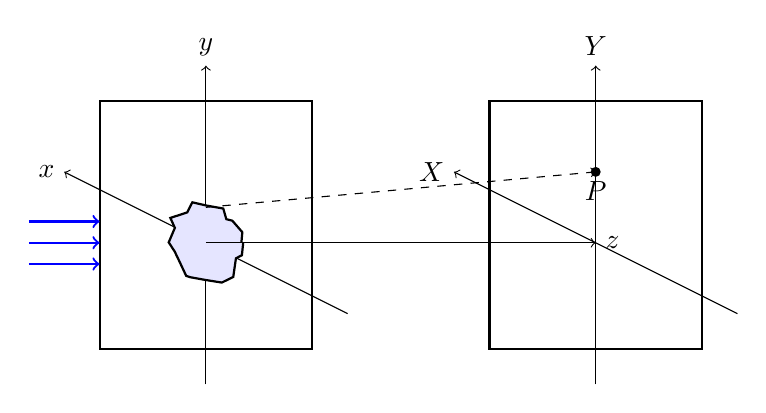
\begin{tikzpicture}[scale=0.9]
		% Плоскость 1 (отверстие)
		\draw[thick] (-2, -1.5) rectangle (1, 2);
		\draw[->] (-0.5, -2) -- (-0.5, 2.5) node[above] {$y$};
		\draw[->] (1.5, -1) -- (-2.5, 1) node[left] {$x$};
		
		\draw[thick, fill=blue!10, decorate, decoration={random steps,segment length=4pt,amplitude=2pt}] (-0.5, 0) circle (0.5);
		
		\draw[->, thick, blue] (-3, 0) -- (-2, 0);
		\draw[->, thick, blue] (-3, 0.3) -- (-2, 0.3);
		\draw[->, thick, blue] (-3, -0.3) -- (-2, -0.3);
		
		% Плоскость 2 (экран)
		\begin{scope}[xshift=5cm]
			\draw[thick] (-1.5, -1.5) rectangle (1.5, 2);
			\draw[->] (0, -2) -- (0, 2.5) node[above] {$Y$};
			\draw[->] (2, -1) -- (-2, 1) node[left] {$X$};
			\fill (0, 1) circle (2pt) node[below] {$P$};
		\end{scope}
		
		\draw[->] (-0.5, 0) -- (5, 0) node[right] {$z$};
		\draw[->, dashed] (-0.5, 0.5) -- (5, 1);
	\end{tikzpicture}
\end{figure}

\begin{align*}
	& K(\alpha) \sim \cos \alpha_0 + \cos \alpha_1 \sim 2 \\
	& \alpha_0 = 0 \qquad \alpha_1 \to 0
\end{align*}
\vspace{-1.5cm}
\begin{align*}
	E(x,y,z) &\sim \iint dx dy \underbrace{E_0 t(x,y)}_{E'} \frac{e^{ikr}}{r} K(\alpha) \sim \frac{2E_0}{d} \iint dx dy \, t(x,y) e^{ikr}
\end{align*}

\begin{align*}
	r &= \sqrt{z^2 + (X-x)^2 + (Y-y)^2} = z \sqrt{1 + \frac{(X-x)^2}{z^2} + \frac{(Y-y)^2}{z^2}} \approx \\
	&\approx z \qty(1 + \frac{1}{2} \frac{X^2 - 2xX + x^2}{z^2} + \frac{1}{2} \frac{Y^2 - 2yY + y^2}{z^2}) = \\
	&= z \qty(1 + \frac{1}{2}\frac{X^2+Y^2}{z^2} + \frac{1}{2} \frac{x^2+y^2}{z^2} - \frac{Xx+Yy}{z^2}) \approx \\
	&\approx z \qty(1 + \frac{X^2+Y^2}{z^2}) - \frac{Xx+Yy}{z}
\end{align*}

\begin{align*}
	E(x,y,z) &\sim \frac{2E_0}{d} \iint dx dy \cdot t(x,y) e^{ikr} \sim \\
	&\sim \text{const} \frac{2E_0}{d} \iint dx dy \, t(x,y) e^{-ik \frac{(Xx + Yy)}{z}}
\end{align*}

Обозначим: $\frac{X}{z} \approx \sin \alpha_x, \quad \frac{Y}{z} = \tg \alpha_y \approx \sin \alpha_y \quad (\alpha_y \to 0)$.

\begin{nb}
	\begin{equation*}
		E(x,y,z) \sim E_0 \iint dx dy \cdot t(x,y) e^{-ik(x \sin\alpha_x + y \sin\alpha_y)}
	\end{equation*}
\end{nb}

\begin{minipage}{0.4\textwidth}
	\begin{align*}
		E(t) &\sim \int E(\omega) e^{-i\omega t} dt \qquad \omega = \frac{2\pi}{T} \\
		E(r) &\sim \int E(k) e^{-ikr} dr \qquad k = \frac{2\pi}{\lambda}
	\end{align*}
\end{minipage}
\begin{minipage}{0.5\textwidth}
	\begin{tikzpicture}
		\draw[->] (-2,0) -- (2,0) node[right] {$k$};
		\draw[->] (0,-0.5) -- (0,1.5) node[above] {$E$};
		\draw[thick, blue] (-1.5,0) sin (-1, 0.3) cos (-0.5, 0) sin (0, 1.2) cos (0.5, 0) sin (1, 0.3) cos (1.5, 0);
		\fill (0,1.2) circle (1.5pt);
		\node[align=left, text width=4cm] at (4, 1) {низкие $k$ - общие черты предмета \\ $k = \frac{2\pi}{\lambda}$};
	\end{tikzpicture}
\end{minipage}

\section{Дифракция на периодической структуре. Простейшая дифракционная решетка}

\begin{figure}[H]
	\centering
	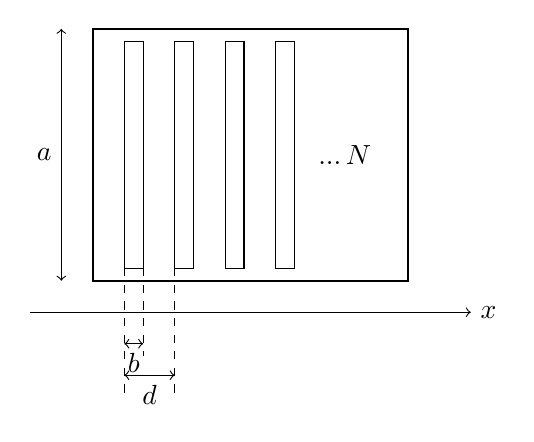
\begin{tikzpicture}[scale=0.8]
		% Решетка
		\draw[thick] (0, -2) rectangle (5, 2);
		\draw[fill=white] (0.5, -1.8) rectangle (0.8, 1.8);
		\draw[fill=white] (1.3, -1.8) rectangle (1.6, 1.8);
		\draw[fill=white] (2.1, -1.8) rectangle (2.4, 1.8);
		\draw[fill=white] (2.9, -1.8) rectangle (3.2, 1.8);
		\node at (4, 0) {$... \, N$};
		
		\draw[<->] (-0.5, -2) -- (-0.5, 2) node[midway, left] {$a$};
		\draw[->] (-1, -2.5) -- (6, -2.5) node[right] {$x$};
		
		\draw[<->] (0.5, -3) -- (0.8, -3) node[midway, below] {$b$};
		\draw[<->] (0.5, -3.5) -- (1.3, -3.5) node[midway, below] {$d$};
		
		\draw[dashed] (0.8, -1.8) -- (0.8, -3.2);
		\draw[dashed] (0.5, -1.8) -- (0.5, -3.8);
		\draw[dashed] (1.3, -1.8) -- (1.3, -3.8);
	\end{tikzpicture}
\end{figure}

\begin{itemize}
	\item наносят $\sim 1200$ штрихов
	\item общие размеры $\sim 10 \si{\centi\meter}$
	\item на всю длину $\sim 10^5$ штрихов
	\item $L \le 10 \si{\centi\meter}$
	\item $a \gg b$
	\item $N \sim 10^5$ штрихов
	\item $-\infty < Y < +\infty$
	\item $b$ -- ширина штриха
	\item $d$ -- период решетки
\end{itemize}

\textbf{Функция пропускания решетки:} 
\[ t(x,y) = \sum_{m=0}^{N} \text{rect}\qty(\frac{X - md}{b}) \leftarrow \text{количество промежутков} \]
(из зарубежной литературы).

\begin{align*}
	E(\alpha_x, \alpha_y) &= E(\alpha_x) \equiv E(\varphi) \sim E_0 \iint dx dy \sum_{m=0}^{N} \text{rect}\qty(\frac{X - md}{b}) \exp{ik(X\sin\alpha_x + Y\sin\alpha_y)} = \\
	&= E_0 \int_{-\infty}^{\infty} dy \, e^{-ik Y \sin\alpha_y} \sum_{m=0}^{N} \int_{md - \frac{b}{2}}^{md + \frac{b}{2}} dx \, e^{-ikX\sin\alpha_x} \sim \\
	&\sim E_0 \sum_{m=0}^{N} \int_{md - \frac{b}{2}}^{md + \frac{b}{2}} dx \exp{-ikX\sin\varphi} \sim E_0 \sum_{m=0}^{N} \int_{-\frac{b}{2}}^{\frac{b}{2}} d\mathcal{X} \exp{-ik(\mathcal{X}+md)\sin\varphi} = \\
	&= E_0 \sum_{m=0}^{N} \qty( \int_{-\frac{b}{2}}^{\frac{b}{2}} d\mathcal{X} e^{-ik\mathcal{X}\sin\varphi} ) e^{-ikmd\sin\varphi}
\end{align*}

Введем новую переменную: $\mathcal{X} = X - md$.
\begin{align*}
	&= \underbrace{E_0 \int_{-\frac{b}{2}}^{\frac{b}{2}} d\mathcal{X} e^{-ik\mathcal{X}\sin\varphi}}_{\sim E_0 \frac{\sin\qty[\frac{k}{2} b \sin\varphi]}{\frac{k}{2}\sin\varphi}} \cdot \sum_{m=0}^{N} e^{-ikmd\sin\varphi} \sim E_0 \frac{\sin\qty[\frac{\pi b}{\lambda}\sin\varphi]}{\frac{\pi b}{\lambda}\sin\varphi} \sum_{m=0}^{N} e^{-ikmd\sin\varphi} \implies
\end{align*}

\begin{equation*}
	E_1(\varphi) \cdot \sum_{m=0}^{N} e^{-ikmd\sin\varphi} = E_1(\varphi) \cdot \frac{1 - \exp{-ikNd\sin\varphi}}{1 - \exp{-ikd\sin\varphi}} = E_1(\varphi) \cdot \frac{\exp{i \frac{k}{2} Nd\sin\varphi} \qty( e^{\frac{i}{2}kNd\sin\varphi} - e^{-\frac{i}{2}kNd\sin\varphi} )}{\exp{i \frac{k}{2} d\sin\varphi} \qty( e^{\frac{i}{2}kd\sin\varphi} - e^{-\frac{i}{2}kd\sin\varphi} )} \implies
\end{equation*}

\begin{equation*}
	\implies E_1(\varphi) \cdot \frac{\exp{- \frac{i}{2}kNd\sin\varphi}}{\exp{- \frac{i}{2}kd\sin\varphi}} \cdot \frac{\sin\qty(\frac{1}{2}kNd\sin\varphi)}{\sin\qty(\frac{1}{2}kd\sin\varphi)} \sim E_0 \frac{\sin\qty(\pi N \frac{d}{\lambda} \sin\varphi)}{\sin\qty(\pi \frac{d}{\lambda} \sin\varphi)} \cdot \mathcal{X}
\end{equation*}

\begin{nb}
	$I = E E^*$ \\ $k = \frac{2\pi}{\lambda}$
	\begin{equation}
		I(x) = I(\varphi) = I_0 \cdot \underbrace{\frac{\sin^2\qty[\frac{\pi b}{\lambda}\sin\varphi]}{\qty[\frac{\pi b}{\lambda}\sin\varphi]^2}}_{\substack{\text{дифракция} \\ \text{на одной} \\ \text{щели}}} \cdot \underbrace{\frac{\sin^2\qty[\pi N \frac{d}{\lambda}\sin\varphi]}{\sin^2\qty[\pi \frac{d}{\lambda}\sin\varphi]}}_{\text{интерференция}}
	\end{equation}
\end{nb}

\begin{figure}[H]
	\centering
	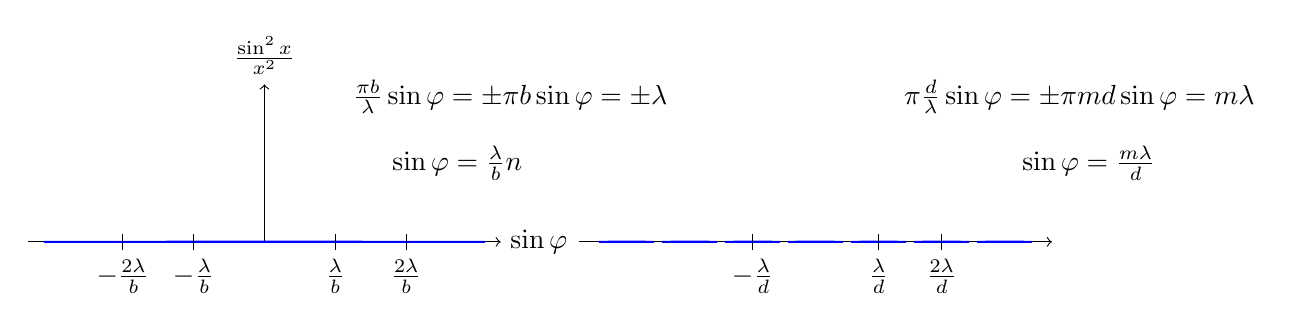
\begin{tikzpicture}
		% First graph (single slit envelope)
		\begin{scope}[shift={(0,0)}]
			\draw[->] (-3, 0) -- (3, 0) node[right] {$\sin\varphi$};
			\draw[->] (0, 0) -- (0, 2) node[above] {$\frac{\sin^2 x}{x^2}$};
			\draw[thick, blue, samples=100, domain=-2.8:2.8] plot (\x, {1.5*(sin(\x*100)/(\x*100))^2});
			
			\draw (-1.8, 0.1) -- (-1.8, -0.1) node[below] {$-\frac{2\lambda}{b}$};
			\draw (-0.9, 0.1) -- (-0.9, -0.1) node[below] {$-\frac{\lambda}{b}$};
			\draw (0.9, 0.1) -- (0.9, -0.1) node[below] {$\frac{\lambda}{b}$};
			\draw (1.8, 0.1) -- (1.8, -0.1) node[below] {$\frac{2\lambda}{b}$};
			
			\node[above right] at (1, 1.5) {$\frac{\pi b}{\lambda} \sin\varphi = \pm \pi \implies b\sin\varphi = \pm \lambda$};
			\node[right] at (1.5, 1) {$\sin\varphi = \frac{\lambda}{b} n$};
		\end{scope}
		
		% Second graph (interference comb)
		\begin{scope}[shift={(7,0)}]
			\draw[->] (-3, 0) -- (3, 0);
		\foreach \x in {-2.4, -1.6, -0.8, 0, 0.8, 1.6, 2.4} {
			\draw[thick, blue, samples=50, variable=\tmp, domain=-0.35:0.35] plot ({\x+\tmp}, {1.5*(sin(\tmp*500)/(\tmp*500))^2});
		}
			\draw (-0.8, 0.1) -- (-0.8, -0.1) node[below] {$-\frac{\lambda}{d}$};
			\draw (0.8, 0.1) -- (0.8, -0.1) node[below] {$\frac{\lambda}{d}$};
			\draw (1.6, 0.1) -- (1.6, -0.1) node[below] {$\frac{2\lambda}{d}$};
			
			\node[above right] at (1, 1.5) {$\pi \frac{d}{\lambda} \sin\varphi = \pm \pi m \implies d\sin\varphi = m\lambda$};
			\node[right] at (2.5, 1) {$\sin\varphi = \frac{m\lambda}{d}$};
		\end{scope}
	\end{tikzpicture}
\end{figure}

Т.к. $d > b$, то быстро осциллирует.
\[ I_0 \lim \frac{\sin^2\qty[\pi N \frac{d}{\lambda}\sin\varphi]}{\sin^2\qty[\pi \frac{d}{\lambda}\sin\varphi]} \sim I_0 \lim \frac{\qty[\pi N \frac{d}{\lambda}\sin\varphi]^2}{\qty[\pi \frac{d}{\lambda}\sin\varphi]^2} \sim I_0 N^2 \]
при $\pi \frac{d}{\lambda}\sin\varphi \to \pi m$.

\begin{figure}[H]
	\centering
	\begin{tikzpicture}
		\begin{scope}[shift={(0,0)}]
			\draw[->] (-3.5, 0) -- (3.5, 0) node[right] {$\sin\varphi$};
			\draw[->] (0, 0) -- (0, 2.5) node[above] {$y$};
			
			% Envelope
			\draw[dashed, red, samples=100, domain=-3.2:3.2] plot (\x, {2*(sin(\x*50)/(\x*50))^2});
			
			% Combined
			\foreach \x in {-2.4, -1.6, -0.8, 0, 0.8, 1.6, 2.4} {
				\draw[thick, blue, samples=50, domain=-0.35:0.35] plot (\x+\x, {2*(sin(\x*50)/(\x*50))^2 * (sin(\x*500)/(\x*500))^2}); % Approximation for visual
			}
			
			\draw[thick, blue] (-2.4, 0) -- (-2.4, 0.8);
			\draw[thick, blue] (-1.6, 0) -- (-1.6, 1.5);
			\draw[thick, blue] (-0.8, 0) -- (-0.8, 1.8);
			\draw[thick, blue] (0, 0) -- (0, 2);
			\draw[thick, blue] (0.8, 0) -- (0.8, 1.8);
			\draw[thick, blue] (1.6, 0) -- (1.6, 1.5);
			\draw[thick, blue] (2.4, 0) -- (2.4, 0.8);
			
			% Ticks
			\draw (-1.6, 0.1) -- (-1.6, -0.1) node[below] {$-\frac{\lambda}{b}$};
			\draw (1.6, 0.1) -- (1.6, -0.1) node[below] {$\frac{\lambda}{b}$};
			\draw (0.8, 0.1) -- (0.8, -0.1) node[below] {$\frac{\lambda}{d}$};
			\draw (2.4, 0.1) -- (2.4, -0.1) node[below] {$\frac{2\lambda}{d}$};
		\end{scope}
		
		\node[fill=green!20, rounded corners, inner sep=5pt] at (3, 2.5) {условие главных max: $d\sin\varphi = \lambda m$};
		\node[fill=green!20, rounded corners, inner sep=5pt] at (3, -1) {условие доп. min: $b\sin\varphi = \lambda n$};
	\end{tikzpicture}
\end{figure}

\begin{itemize}
	\item $\frac{d}{b} = \frac{m}{n}$
\end{itemize}

\subsection*{Дифракционная решетка как спектральный прибор}

$\sin\varphi = \frac{\lambda}{d} m \implies \sin\varphi \sim \lambda \implies$ разложение в спектр $\qty(\sin\varphi = \frac{k}{z})$

\textbf{Особенности спектра:}
\begin{enumerate}
	\item $m=0, x=0$
	\item при фиксированном $m, d$, чем больше $\lambda$, тем больше $\sin\varphi \implies$ далее от центра линий с наименьш. $\lambda$ возникают первыми
	\item ширина между линиями во 2-ом и далее порядков больше, чем в первом ($\sin\varphi \sim m$), поэтому при увеличении порядка может получаться так, что фиолетовая линия ($m-1$) порядка будет накладываться на красную линию $m$ порядка
	\item с ростом $m$ интенсивность света уменьшается
\end{enumerate}

\textbf{Характеристики спектрального прибора:}
\begin{enumerate}
	\item \underline{Область свободной дисперсии} --- ширина области спектра, на которую не наклад. соседние порядки.
	\[ m(\lambda + \Delta \lambda) = (m+1)\lambda \implies \Delta \lambda = \frac{\lambda}{m} \]
	
	\item \underline{Угловая дисперсия}: $D = \frac{d\varphi}{d\lambda}$ --- характеризует степень пространств. или углового разделения с длинами волн, отлич. на $d\lambda$.
	\[ \cos\varphi d\varphi = \frac{m}{d} d\lambda \implies D = \frac{d\varphi}{d\lambda} = \frac{m}{d\cos\varphi} \]
	
	\item \underline{Разрешающая способность} ($R$): $R = \frac{\lambda}{\delta \lambda}$, $\delta \lambda$ --- наименьшая разность длин волн спектральных линий, при которой эти линии еще воспринимаются прибором.
	
	\underline{Критерий Релея:} $\to$ спектр. линии считаются разрешенными, если главный max одной СЛ совпадает с первым min другой.
	
	\begin{minipage}{0.2\textwidth}
		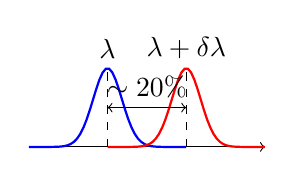
\begin{tikzpicture}
			\draw[->] (-1.5, 0) -- (1.5, 0);
			\draw[thick, blue, samples=50, domain=-1.5:0.5] plot (\x, {exp(-(\x+0.5)*(\x+0.5)*15)});
			\draw[thick, red, samples=50, domain=-0.5:1.5] plot (\x, {exp(-(\x-0.5)*(\x-0.5)*15)});
			\draw[dashed] (-0.5, 0) -- (-0.5, 1) node[above] {$\lambda$};
			\draw[dashed] (0.5, 0) -- (0.5, 1) node[above] {$\lambda+\delta\lambda$};
			\draw[<->] (-0.5, 0.5) -- (0.5, 0.5) node[midway, above] {$\sim 20\%$};
		\end{tikzpicture}
	\end{minipage}
	\begin{minipage}{0.7\textwidth}
		\begin{equation*}
			\begin{cases}
				(\lambda + \delta \lambda)m = d\sin\varphi \quad \text{--- max} \\
				\qty(m + \frac{1}{N})\lambda = d\sin\varphi \quad \text{--- 1ый min $m$-ого порядка}
			\end{cases} \implies \frac{\lambda}{\delta \lambda} = mN
		\end{equation*}
	\end{minipage}
\end{enumerate}

\section{16.04 Классическая теория излучения электромагнитных волн}

\begin{itemize}
	\item $j = nq\vb{v}$ \\
	ускоренные движущиеся заряды порождают электромагнитное поле
\end{itemize}

\begin{figure}[H]
	\centering
	\begin{tikzpicture}[scale=0.9]
		\draw[thick] (-2, 0) -- (0, 0);
		\filldraw (0,0) circle (2pt) node[below] {$q$};
		\draw[blue, thick, ->] (0,0) to[out=135, in=0] (-1, 0.5) to[out=180, in=90] (-2, 0) to[out=270, in=180] (-1, -0.5) to[out=0, in=225] (0,0);
		\draw[blue, thick, ->] (0,0) to[out=45, in=180] (1, 0.5) to[out=0, in=90] (2, 0) to[out=270, in=0] (1, -0.5) to[out=180, in=315] (0,0);
		\node at (-1.5, 0.8) {$\vb{B}$};
		\node at (-1.5, -0.8) {$\vb{E}$};
		
		\begin{scope}[shift={(6, 0)}]
			\draw[->] (-1, -2) -- (-1, 2) node[left] {$v$};
			\draw[->] (-1.5, -1.5) -- (3, -1.5) node[below] {$t$};
			\draw[thick, red] (-1, -1.5) -- (0, -1.5) -- (1, 0) -- (3, 0);
			\node[below] at (0, -1.5) {$0$};
			\node[below] at (1, -1.5) {$\tau$};
			\node[below] at (2.5, -1.5) {$t \gg \tau$};
			\node[left] at (-1, 0) {$v \ll c$};
			
			\node[align=left, text width=4cm] at (0, -3) {$\tau \ll t$ \\ $t = \frac{R}{c}$ -- время, за которое мы узнаем, что движется заряд.};
		\end{scope}
	\end{tikzpicture}
\end{figure}

Поле ускоренно движущегося заряда:

\begin{figure}[H]
	\centering
	\begin{tikzpicture}[scale=1.5]
		\draw[thick, blue] (0,0) circle (1.5);
		\draw[thick, blue] (0,0) circle (1.3);
		\filldraw (0,0) circle (1.5pt) node[below left] {$q$};
		
		\foreach \angle in {0, 45, 90, 135, 180, 225, 270, 315} {
			\draw[->, dashed] (0,0) -- (\angle:1.3);
			\draw[->, thick, red] (\angle:1.3) -- (\angle-10:1.5);
			\draw[->] (\angle-10:1.5) -- (\angle-10:2);
		}
		
		\node[align=left, text width=3.5cm] at (2.5, 1) {излом линий - сигнал, дошедший до наблюдателя};
		\node[align=left, text width=3.5cm] at (2.5, -1) {начало равноускоренного движения (наблюд. не знают)};
		\node[align=left, text width=3.5cm] at (-0.5, -1.8) {сфера, где наблюдатели знают, что равномер. движение};
		
		\begin{scope}[shift={(-3.5, 0)}]
			\draw[thick, blue] (0, -1) arc (270:90:1);
			\draw[thick, blue] (0.5, -1) arc (270:90:1);
			\draw[->] (0, 0) -- (2, 0.5);
			\draw[->] (0, 0) -- (0, 1) node[above] {$\vb{E}_n$};
			\draw[->, red, thick] (0.8, 0.2) -- (0.5, 0.7) node[above] {$\vb{E}_\tau$};
			\draw[->, thick] (0.8, 0.2) -- (1.2, 0.3) node[right] {$\vb{E}$};
			
			\draw[dashed] (0,0) -- (0.8, 0.2);
			\node[left] at (0, 0) {$vt$};
			\draw[<->] (0.2, 0) -- (0.2, 0.8) node[midway, right] {$v\tau \sin\theta$};
			\draw[<->] (0, -0.2) -- (0.5, -0.2) node[midway, below] {$c\tau$};
			
			\node at (1.5, -1) {$\frac{E_\tau}{E_n} = \frac{v\tau \sin\theta}{c\tau}$};
			\node[align=left, text width=3.5cm] at (0, -2) {момент времени, где случился излом и началось равномерное движение};
		\end{scope}
	\end{tikzpicture}
\end{figure}

получили из подобия:
\begin{equation*}
	\Downarrow
\end{equation*}
\begin{equation*}
	E_\tau = E_n \cdot \frac{vt\sin\theta}{c\tau} \qquad E_n = \frac{1}{4\pi\varepsilon_0} \frac{q}{R^2} \text{ --- поле точечного заряда}
\end{equation*}

\begin{itemize}
	\item Обобщим, что заряд движется с переменным ускорением рядом с началом координат $a(t') = a(t - \frac{R}{c})$.
	$t'$ -- время, за которое сигнал будет до нас доходить.
	\begin{equation*}
		E_\tau = \frac{1}{4\pi\varepsilon_0} \frac{q}{R^2} \cdot \frac{a \tau t \sin\theta}{c\tau} = \frac{1}{4\pi\varepsilon_0} \frac{q a \sin\theta}{c^2 R} \sim \frac{1}{R}
	\end{equation*}
	$\theta = \frac{\pi}{2} / \theta = 0 \to E_\tau = 0$ не излучает (в направлении движения). На экваторе: $E_\tau = \text{max}$.
	(2) поле $E_\tau \sim \sin\theta$, $\theta$ -- угол между ускорением и расстоянием ($\theta = \widehat{\vb{a}, \vb{R}}$). В разных направлениях -- разное.
\end{itemize}

\begin{nb}
	\begin{equation*}
		E = \frac{1}{4\pi\varepsilon_0} \frac{q \cdot a(t - \frac{R}{c}) \sin\theta}{c^2 R}
	\end{equation*}
	если $a$ меняется по косинусу, это будет сферическая волна (кривая сферическая волна).
	т.е. еще раз: 1) $\theta = 0, \pi \to E_\tau = 0$, 2) $\theta = \frac{\pi}{2} \to E_\tau = \text{max}$.
\end{nb}

\subsection*{Модель атома Томсона}

$|q_e| = |q_+|$ --- система нейтральна. Это модель одна из лучших.
\begin{figure}[H]
	\centering
	\begin{tikzpicture}
		\draw[thick] (0,0) circle (1.5);
		\node at (0, 0.5) {$+$}; \node at (0.5, 0) {$+$}; \node at (-0.5, 0) {$+$}; \node at (0, -0.5) {$+$};
		\node at (0.8, 0.8) {$-$}; \node at (-0.8, -0.8) {$-$};
		
		\begin{scope}[shift={(4,0)}]
			\draw[thick] (0,0) circle (1.5);
			\draw[dashed] (0,0) circle (0.8);
			\draw[->] (0,0) -- (0.8, 0) node[midway, below] {$r$};
			\draw[->] (0,0) -- (0, 1.5) node[midway, right] {$R_0$};
			\filldraw (0.8, 0) circle (1.5pt) node[right] {$q_-$};
			\node at (-1, 1) {облако отриц. заряда};
			\node at (-2, 0) {смещение электр. оболочки от-но ядра};
			\draw[->] (-2.5, -0.5) -- (-1.5, 0);
		\end{scope}
	\end{tikzpicture}
\end{figure}

По th Гаусса: $\oint \vb{E} d\vb{S} = \frac{q_{\text{вн}}}{\varepsilon_0}$
\begin{align*}
	q_{\text{вн}} = \rho V_{\text{вн}} = \frac{q}{V} V_{\text{внутри}} \qquad E \cdot S = \frac{q_{\text{вн}}}{\varepsilon_0} \\
	q_{\text{вн}} = \frac{q}{\frac{4}{3}\pi R_0^3} \cdot \frac{4}{3}\pi r^3 \qquad E \cdot 4\pi r^2 = \frac{1}{\varepsilon_0} q \frac{r^3}{R_0^3} \\
	q_{\text{вн}} = q \cdot \frac{r^3}{R_0^3} \qquad \implies \vb{E} = - \frac{1}{4\pi\varepsilon_0} \frac{q}{R_0^3} \vb{r}
\end{align*}

$\vb{F} = q\vb{E} = - \frac{1}{4\pi\varepsilon_0} \frac{q^2}{R_0^3} \vb{r}$

По II закону Ньютона:
\begin{align*}
	m \cdot \frac{d^2\vb{r}}{dt^2} &= - \frac{1}{4\pi\varepsilon_0} \frac{q^2}{R_0^3} \vb{r} \\
	m \cdot \frac{d^2\vb{r}}{dt^2} &+ \frac{1}{4\pi\varepsilon_0} \frac{q^2}{R_0^3} \vb{r} = 0
\end{align*}
уравнение гармонических колебаний: $\frac{d^2\vb{r}}{dt^2} + \omega_0^2 \vb{r} = 0$.
Решение: $\vb{r}(t) = \vb{r}_0 \exp{i\omega_0 t}$.
\begin{nb}
	$\omega_0 = \sqrt{\frac{q^2}{4\pi\varepsilon_0 m R_0^3}}$ --- резонансная частота (частота электрон. колебаний).
\end{nb}

\begin{itemize}
	\item $\vb{p}(t) = \vb{p}_0 \exp{i\omega_0 t}$ ($\vb{p} = q\vb{r}(t)$) --- осциллирующий диполь.
	\item $q \cdot \vb{a} = q\ddot{\vb{r}} = \ddot{\vb{p}}$ \quad $E = \frac{1}{4\pi\varepsilon_0} \frac{\ddot{p} \sin\theta}{c^2 R}$ --- поле осциллирующего диполя.
	\item $\ddot{\vb{p}} = (i\omega_0)^2 \vb{p}_0 \exp{i\omega_0 t}$.
	\item $E = \frac{1}{4\pi\varepsilon_0} \qty( (i\omega_0)^2 \frac{p_0 \exp{i\omega_0 t}}{c^2 R} \sin\theta ) = - \frac{1}{4\pi\varepsilon_0} \frac{p_0 \omega_0^2 \sin\theta}{c^2 R} \exp{i\omega_0 t}$ --- сферическая волна.
	\item $I = \sqrt{\frac{\varepsilon_0}{\mu_0}} E E^* = \frac{1}{\mu_0 c} E E^* = \frac{1}{\mu_0 c} \frac{1}{16\pi^2\varepsilon_0^2} \frac{p_0^2 \omega_0^4 \sin^2\theta}{c^4 R^2} = \frac{1}{16\pi^2\varepsilon_0} \frac{p_0^2 \omega_0^4 \sin^2\theta}{c^3 R^2}$.
\end{itemize}

\begin{nb}
	\begin{equation}
		I = \frac{1}{16\pi^2\varepsilon_0} \frac{p_0^2 \omega_0^4 \sin^2\theta}{c^3 R^2} \qquad \text{дипольное излучение}
	\end{equation}
\end{nb}
рассматриваем дальние расстояния $\implies$ используем ф-лы для плоской волны $I = \langle S \rangle_T, \vb{S} = [\vb{E}, \vb{H}], H = \frac{B}{\mu_0}, E=cB$ --- для плоской волны.

Все определяется второй производной дипольного момента.

\begin{itemize}
	\item \textbf{Диаграмма направленности:}
	\begin{figure}[H]
		\centering
		\begin{tikzpicture}
			\draw[->] (0,-1.5) -- (0,2) node[right] {$z$};
			\draw[->] (-3,0) -- (3,0);
			\draw[thick, red, domain=0:360, samples=100] plot ({2*sin(\x)*sin(\x)*cos(\x)}, {2*sin(\x)*sin(\x)*sin(\x)});
			\draw[->, thick, blue] (0,0) -- (1, 1) node[midway, above left] {$\theta$};
			\node[right] at (1, 0.5) {$I = \text{max}$};
			\node[below right] at (0, -1) {тор};
		\end{tikzpicture}
	\end{figure}
\end{itemize}